%%=============================================================================
%% Methodologie
%%=============================================================================

\chapter{Methodologie}
\label{ch:methodologie}

%% TODO: Hoe ben je te werk gegaan? Verdeel je onderzoek in grote fasen, en
%% licht in elke fase toe welke stappen je gevolgd hebt. Verantwoord waarom je
%% op deze manier te werk gegaan bent. Je moet kunnen aantonen dat je de best
%% mogelijke manier toegepast hebt om een antwoord te vinden op de
%% onderzoeksvraag.

In dit hoofdstuk wordt beschreven hoe er te werk is gegaan om een correct antwoord te vinden op de onderzoeksvragen.

We gaan van start met een requirements analyse. Daarna gaan we kijken hoe actief de community is rond deze twee frameworks en welke libraries reeds door de community werden geïnstrumenteerd. Vervolgens gaan we voor beide tools een proof-of-concept opzetten om aan te tonen hoe we deze kunnen implementeren in een project.

\section{Requirements analyse}
Via de requirements analyse gaan we na aan welke functionele en niet functionele requirements de frameworks moeten voldoen om deze succesvol in de stack van XTi te kunnen implementeren. In eerste instantie gaan we bekijken aan welke functionele requirements moet worden voldaan. Daarna lijsten we de niet functionele requirements op.

\subsection{Functionele requirements}
\begin{itemize}
	\item Vergaren van span data
	\item Span data word geaggregeerd in traces
	\item Traces zijn exporteerbaar naar verschillende backends
	\item Ondersteuning voor Java
\end{itemize}

\subsection{Niet functionele requirements}
\begin{itemize}
	\item Minimale impact op code base
	\item Minimale impact op performantie
	\item Grote betrouwbaarheid
	\item Mogelijkheid om eenvoudig over te schakelen naar een andere backend
\end{itemize}

\section{Onderzoek naar de community}
Om na te gaan hoe actief de community is voor elke standaard gaan we de desbetreffende github repositories vergelijken. We gaan ons voornamelijk op de Java en JavaScript repositories toespitsen. Implementaties voor andere programmeertalen zijn voor dit onderzoek van geen belang.

We gaan voor elke standaard na hoeveel forks, pull requests en contributors er zijn voor de desbetreffende libraries, op die manier kunnen we een beeld schetsen over de community en hoe actief ze al dan niet is. In tabel \ref{tbl:opentracingcontrib} zien we de statistieken van de OpenTracing repositories\footnote{https://github.com/opentracing} voor de Java en JavaScript implementaties. In tabel \ref{tbl:opencensuscontrib} zien we de statistieken voor de OpenCensus repositories\footnote{https://github.com/census-instrumentation} van de Java en Node.js implementaties. Zoals we kunnen zien zijn voor de Java implementatie, met uitzondering van het aantal pull requests, vergelijkbare contributies te zien. Ook voor de JavaScript, respectievelijk Node.js voor OpenCensus, zien we gelijkaardige resultaten.

Verder kijken we naar de contribution repositories voor OpenTracing\footnote{https://github.com/opentracing-contrib} en OpenCensus\footnote{https://github.com/census-instrumentation/opencensus-java/tree/master/contrib}. Dit zijn de repositories waar de community hun geïnstrumenteerde libraries of add-ons kunnen toevoegen. In tabel \ref{tbl:instrumented_libraries} zien we een overzicht van de reeds geïnstrumenteerde Java libraries door de community voor beide frameworks. Zoals we kunnen zien is op dit gebied de OpenTracing community een flink stuk actiever. Op het moment van schrijven zijn er voor OpenTracing maar liefst 30 Java libraries die door de community geïnstrumenteerd werden. Dit tegenover slechts 6 Java libraries voor OpenCensus.
\begin{table}
	\caption{GitHub statistieken OpenTracing van 13-12-2015 tot en met 01-01-2019}
	\label{tbl:opentracingcontrib}
	\begin{center}
		\begin{tabular}{| p{5cm} | l | l | l |}
			\hline
			Library & Aantal forks & Aantal pull requests & Aantal contributors \\ \hline
			opentracing-java & 197 & 203 & 31 \\ \hline
			opentracing-javascript & 58 & 70 & 21 \\ \hline
		\end{tabular}
	\end{center}
\end{table}
\begin{table}
	\caption{GitHub statistieken OpenCensus van 15-05-2016 tot en met 01-01-2019}
	\label{tbl:opencensuscontrib}
	\begin{center}
		\begin{tabular}{| p{5cm} | l | l | l |}
			\hline
			Library & Aantal forks & Aantal pull requests & Aantal contributors \\ \hline
			opencensus-java & 123 & 1342 & 29 \\ \hline
			opencensus-node & 39 & 188 & 28 \\ \hline
		\end{tabular}
	\end{center}
	
\end{table}
\begin{table}
	\label{tbl:instrumented_libraries}
	\caption{Door de community geïnstrumenteerde libraries}
	\begin{center}
	\begin{tabular}{| p{5cm} | l | l |}
	\hline
	\textbf{Library} & \textbf{OpenTracing} & \textbf{OpenCensus} \\ \hline \hline
	Apache HttpClient & ja & nee \\ \hline
	Apache Kafka & ja & nee \\ \hline
	Apache Thrift & ja & nee \\ \hline
	JDBC & ja & nee \\ \hline
	Redis & ja & nee \\ \hline
	Redisson & ja & nee \\ \hline
	gRPC & ja & ja \\ \hline
	Spring & ja & ja \\ \hline
	JDBI & ja & nee \\ \hline
	JaxRS & ja & nee \\ \hline
	Java Web Servlet & ja & ja \\ \hline
	Elasticsearch Client & ja & nee \\ \hline
	AWS SDK & ja & nee \\ \hline
	Hazelcast & ja & nee \\ \hline
	JMS & ja & nee \\ \hline
	P6Spy & ja & nee \\ \hline
	RabbitMQ & ja & nee \\ \hline
	Java Concurrent library & ja & nee \\ \hline
	Solr client & ja & nee \\ \hline
	RxJava & ja & nee \\ \hline
	Neo4j Driver & ja & nee \\ \hline
	Memcached Client & ja & nee \\ \hline
	Mongo Driver & ja & nee \\ \hline
	Cassandra Driver & ja & nee \\ \hline
	Akka & ja & nee \\ \hline
	OkHttp & ja & nee \\ \hline
	Vert.x web & ja & nee \\ \hline
	CDI (Context and Dependency Injection) & ja & nee \\ \hline
	Dropwizard & ja & ja \\ \hline
	HpROSE & ja & nee \\ \hline
	AppEngine & nee & ja \\ \hline
	Http Jetty Client & nee & ja \\ \hline \hline
	\textbf{Totaal} & 30 & 6 \\ \hline
	\end{tabular}
\end{center}
\end{table}

Zoals reeds vermeld in hoofdstuk \ref{ch:stand-van-zaken} biedt OpenCensus ook out-of-the-box ondersteuning voor het vergaren en exporteren van metrics. Als we wat verder kijken in de contribution repository van OpenTracing vinden we dat de community voor dit framework ook een metrics collector en exporter heeft ontwikkeld voor Java\footnote{https://github.com/opentracing-contrib/java-metrics}.

\section{Proof-of-concept}
In deze sectie gaan we voor beide frameworks een proof-of-concept opstellen. Hierbij gaan we een project aanmaken in Springboot en de te volgen stappen voor beide frameworks beschrijven.

\subsection{OpenTracing}
\subsubsection{Aanmaken root project}
We maken een nieuw maven\footnote{https://maven.apache.org/} project aan in onze IDE \footnote{Voor dit onderzoek wordt steeds gebruik gemaakt van de IntelliJ IDE} en definiëren onze dependencies in de pom file.

Bij OpenTracing kunnen we kiezen voor een dependency die automatisch een tracer configureert voor een bepaalde backend. Er is keuze tussen Jaeger en Zipkin. Dit kan handig zijn indien je op voorhand een keuze maakt voor Jaeger of Zipkin. In dit onderzoek kiezen we om gebruik te maken van de Jaeger backend voor het visualiseren van de traces.

Aangezien we willen ontwikkelen voor een microservicearchitectuur maken we een aparte module aan die de configuratie van onze tracing bevat. Zo kunnen we voor elke service deze module importeren via een dependency. Zo dienen we de configuratie enkel in deze module aan te passen indien we deze willen veranderen. Anders zouden we in geval van aanpassing in elke module (service) deze aanpassingen manueel moeten doorvoeren.

In de root \code{pom.xml} gaan we eerst de dependency management opzetten en onze modules toevoegen, namelijk de configuratie voor de tracing en een microservice module. We defini\"{e}ren tevens dat we wensen gebruik te maken van het \code{spring-boot-starter-parent} project. Dit zorgt ervoor dat we alle nodige dependencies voor een spring-boot project niet zelf moeten declareren. In de root pom defini\"{e}ren we tevens al de versies die we wensen te gebruiken. Zo hebben we slechts \'{e}\'{e}n plaats waar we aanpassingen moeten doen indien we een andere versie wensen te gebruiken.
\codefragment{xml}{../opentracingparent/pom.xml}{Root dependency management en project settings.}{lst:rootpom}

\subsubsection{Aanmaken tracing configuratie module}
Onder het root project maken we een nieuwe module aan voor de configuratie van onze tracing met als parent ons root project. We gebruiken de dependency \code{opentracing-spring-jaeger-cloud-starter} die we in onze root pom hebben gedefinieerd.
\codefragment{XML}{../opentracingparent/opentracing-configuration/pom.xml}{pom.xml voor de tracing configuratie.}{lst:opentracingpom}

Verder dienen we in deze module enkel een configuratie bean te voorzien voor de tracer. We maken een tracer aan met behulp van omgevingsvariabelen. Zo kunnen we voor elke service gemakkelijk de configuratie aanpassen door de waarde van een variabele aan te passen. Dit kan op verschillende manieren, echter gaan we voor dit onderzoek met docker containers\footnote{https://www.docker.com} werken, we kunnen dus voor elke service gemakkelijk de omgevingsvariabelen aanpassen.

\codefragment{java}{../opentracingparent/opentracing-configuration/src/main/java/be/hogent/distributedtracing/tracer/JaegerTracer.java}{Spring configuratie die een bean van een tracer voorziet.}{lst:jaegertracer}

\subsubsection{Aanmaken module voor microservice}
Terug onder het root project maken we een nieuwe module aan met als parent het root project. Deze module zal de microservice bevatten met een eenvoudige \gls{REST} \gls{API}.

We starten terug met het toevoegen van de juiste dependencies aan de pom file. In dit triviale geval zullen we enkel een dependency nodig hebben naar onze \code{opentracing-configuration} module en naar de \code{spring-boot-starter-web} module.

Naast de dependencies gaan we hier ook de build configureren. We maken gebruik van de \code{docker-maven-plugin}\footnote{https://github.com/spotify/docker-maven-plugin}. Deze configuratie zorgt ervoor dat een build van het project automatisch een docker image aanmaakt.

\codefragment{XML}{../opentracingparent/user-service/pom.xml}{pom.xml voor een triviale microservice.}{lst:userservicepom}

Aangezien we een springboot applicatie maken voorzien we een \code{application.yml} om de applicatie parameters te defini\"{e}ren.

\codefragment{java}{../opentracingparent/user-service/src/main/resources/application.yml}{Configuratie van de springboot applicatie. We laten de webservice op poort 3333 draaien.}{lst:userserviceconfig}

Vervolgens maken we de entrypoint aan om de applicatie te kunnen opstarten. Hier importeren we ook de configuratie voor de tracer door middel van de annotatie \code{@Import(JaegerTracer.class)}. We annoteren de klasse met \code{@SpringBootApplication}, zo weet Spring dat het om een spring boot applicatie gaat. Verder dienen we enkel een \code{main} methode toe te voegen. In deze methode starten we de applicatie op door middel van volgende code \code{SpringApplication.run(UserService.class);}.

\codefragment{java}{../opentracingparent/user-service/src/main/java/be/hogent/distributedtracing/UserService.java}{De entrypoint om de applicatie op te starten. Hier importeren we ook onze tracing configuratie.}{lst:userservice}

Er rest ons enkel nog een REST endpoint aan te maken. Het volstaat om volgende klasse aan te maken, spring zorgt voor het aanmaken van een instantie en het beschikbaar stellen van de endpoint.

\codefragment{java}{../opentracingparent/user-service/src/main/java/be/hogent/distributedtracing/controllers/UserController.java}{De REST controller. Springboot zorgt voor het open stellen van de endpoint.}{lst:usercontroller}

\subsubsection{Omgeving opstarten}
Nu we de code geschreven hebben kunnen we deze compileren. In de root directory van het project voeren we het volgende commando uit:
\begin{list}{}{}
	\item \code{mvn clean install}
\end{list}
Dit commando zal de modules compileren en de docker image voor de user service aanmaken\footnote{Let er op dat de Docker engine reeds geïnstalleerd moet zijn op uw development computer}.

Om het ons gemakkelijk te maken, maken we een \code{docker-compose.yml}\footnote{https://docs.docker.com/compose/overview/} file aan met de configuratie voor de docker containers. Dit zorgt ervoor dat met een enkel commando de volledige omgeving wordt geconfigureerd en opgestart.

In een docker-compose configuratie vinden we enkele belangrijke elementen terug. Bovenaan de file wordt de docker-compose versie gespecificeerd. Hieronder gaan we onze services declareren die we via deze file willen configureren en starten.

Iedere service heeft een unieke naam en volgt onmiddellijk na de \code{services:} declaratie. Voor elke service specificeren we de docker image die we wensen te gebruiken. In dit geval \code{jaegertracing/all-in-one:latest} en \code{user-service:latest}. \"{}latest\"{} is de image tag, we vragen hier dus specifiek naar de laatst gepubliceerde versie van de image. Voor onze user service werd deze tag toegekend in listing \ref{lst:userservicepom}. Verder specificeren we voor elke service de hostnaam, de domeinnaam en de te publiceren po(o)rt(en) naar de host machine\footnote{Via deze poorten gaan we later connectie maken met de services}.

Aangezien we in listing \ref{lst:jaegertracer} voor onze user service een tracer aanmaken met de omgevingsvariabelen, moeten we deze variabelen ook in deze file declareren. Dit doen we aan de hand van de \code{environment:} property. Elke variabele die kan gedeclareerd worden om Jaeger van de gewenste configuratie te voorzien wordt opgelijst in tabel \ref{tbl:jaeger}. Voor deze eenvoudige applicatie gebruiken we echter enkel \code{JAEGER\_SERVICE\_NAME}, \code{JAEGER\_AGENT\_HOST} en \code{JAEGER\_SAMPLER\_PARAM}\footnote{We geven de waarde 1 om er voor te zorgen dat elke call naar de service een trace produceert. Doe dit nooit in een productieomgeving}. Dit omdat we gebruik gaan maken van de Docker image van de Jaeger backend en de meeste parameters een gewenste default waarde hebben.

\codefragment{xml}{../opentracingparent/docker/docker-compose.yml}{Inhoud van de docker-compose file}{lst:dockercompose}

Om de omgeving op te starten navigeren we, in een terminal, naar de directory waar de \code{docker-compose.yml} file staat. Het volstaat om in deze directory het commando \code{docker-compose up}\footnote{Indien je met een Unix besturingssysteem werkt is het mogelijk dat u het commando eerst nog dient te installeren} uit te voeren.

\begin{table}
	\label{tbl:jaeger}
	\caption{Omgevingsvariabelen voor configuratie van een Jaeger client}
	\begin{center}
		\scalebox{.85}{
			\begin{tabular}{| l | l | p{5cm} |}
				\hline
				\textbf{Property} & \textbf{Vereist} & \textbf{Omschrijving} \\ \hline
				JAEGER\_SERVICE\_NAME & ja & De naam van de service \\ \hline
				JAEGER\_AGENT\_HOST & nee & De hostnaam waarop de Jaeger instantie draait om te communiceren via UDP \\ \hline
				JAEGER\_AGENT\_PORT & nee & De poort waarop de Jaeger instantie luistert naar inkomende traces \\ \hline
				JAEGER\_ENDPOINT & nee & De traces endpoint voor het geval de client een directe verbinding heeft met de collector, bv. http://jaeger-collector:14268/api/traces \\ \hline
				JAEGER\_AUTH\_TOKEN & nee & Authentication Token om te authenticeren naar de endpoint \\ \hline
				JAEGER\_USER & nee & Username voor basis authenticatie naar de endpoint \\ \hline
				JAEGER\_PASSWORD & nee & Password voor basis authenticatie naar de endpoint \\ \hline
				JAEGER\_PROPAGATION & nee & Comma separated list van trace formats om een trace context te propageren\footnote{Deze optie bestaat om het mogelijk te maken, om traces die via de Zipkin instrumentatie zijn aangemaakt, te propageren naar Jaeger}. Defaults is dit het standaard Jaeger formaat. Geldige waardes zijn jaeger en b3 \\ \hline
				JAEGER\_REPORTER\_LOG\_SPANS & nee & Bepaalt of de loggingreporter ook de spans moet loggen \\ \hline
				JAEGER\_REPORTER\_MAX\_QUEUE\_SIZE & nee & Bepaalt de grootte van de queue voor de loggingreporter \\ \hline
				JAEGER\_REPORTER\_FLUSH\_INTERVAL & nee & Bepaalt de flushinterval voor de loggingreporter in ms. \\ \hline
				JAEGER\_SAMPLER\_TYPE & nee & Het type van de sampler\footnote{https://www.jaegertracing.io/docs/1.8/sampling/\#client-sampling-configuration} \\ \hline
				JAEGER\_SAMPLER\_PARAM & nee & Bepaalt hoe vaak er gesampled wordt. Dit is een numerieke waarde tussen 1 en 0\footnote{Grenzen inbegrepen}. Waarbij 1 staat voor altijd sampelen en 0 voor nooit sampelen. \\ \hline
				JAEGER\_SAMPLER\_MANAGER\_HOST\_PORT & nee & Indien gebruik wordt gemaakt van de remote sampler moet hier de hostname en poort gedefinieerd worden om met de remote sampler te kunnen communiceren \\ \hline
				JAEGER\_TAGS & nee & Een comma separated list om tags te voorzien in de traces. Een tag wordt 	als key-pair meegegeven in de vorm van \code{tagName = value} \\ \hline
			\end{tabular}
		}
	\end{center}
\end{table}

\subsubsection{Verifi"eren van de installatie}
Zowel de ge"instrumenteerde user service als de Jaeger backend collector zijn nu actief. Dit gaan we verifi"eren door te surfen naar \code{http://localhost:5555}. Op deze locatie zien we de user interface van Jaeger. Op dit moment is er nog niet veel te zien, daarom gaan we nu traces genereren.

Om een trace te genereren volstaat het om de endpoint van onze user service aan te roepen. In dit geval is dit \code{users/\{id\}}, \code{id} kan om het even welk getal zijn. Zoals we in listing \ref{lst:dockercompose} hebben opgegeven, is onze service actief op poort \code{3333}. We surfen dus naar \code{http://localhost:3333/users/1234} om een trace te genereren.

We keren nu terug naar de interface van Jaeger. We zien inderdaad in het zoekscherm in figuur \ref{fig:user-service} dat de user-service werd toegevoegd aan de lijst van services. Als we voor deze service nu de traces zoeken zien we in figuur \ref{fig:user-service-trace} inderdaad dat er ook een trace is verschenen.

\begin{figure}
	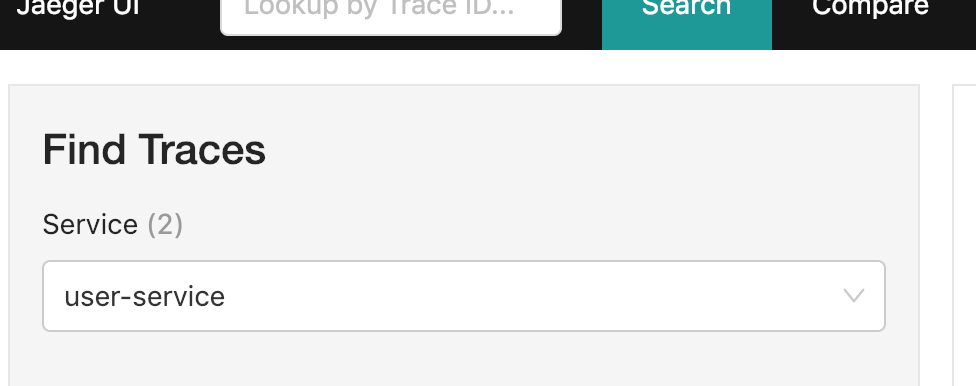
\includegraphics[width=\linewidth]{img/user-service.png}
	\caption{De user-service is in de lijst van services verschenen.}
	\label{fig:user-service}
\end{figure}
\begin{figure}
	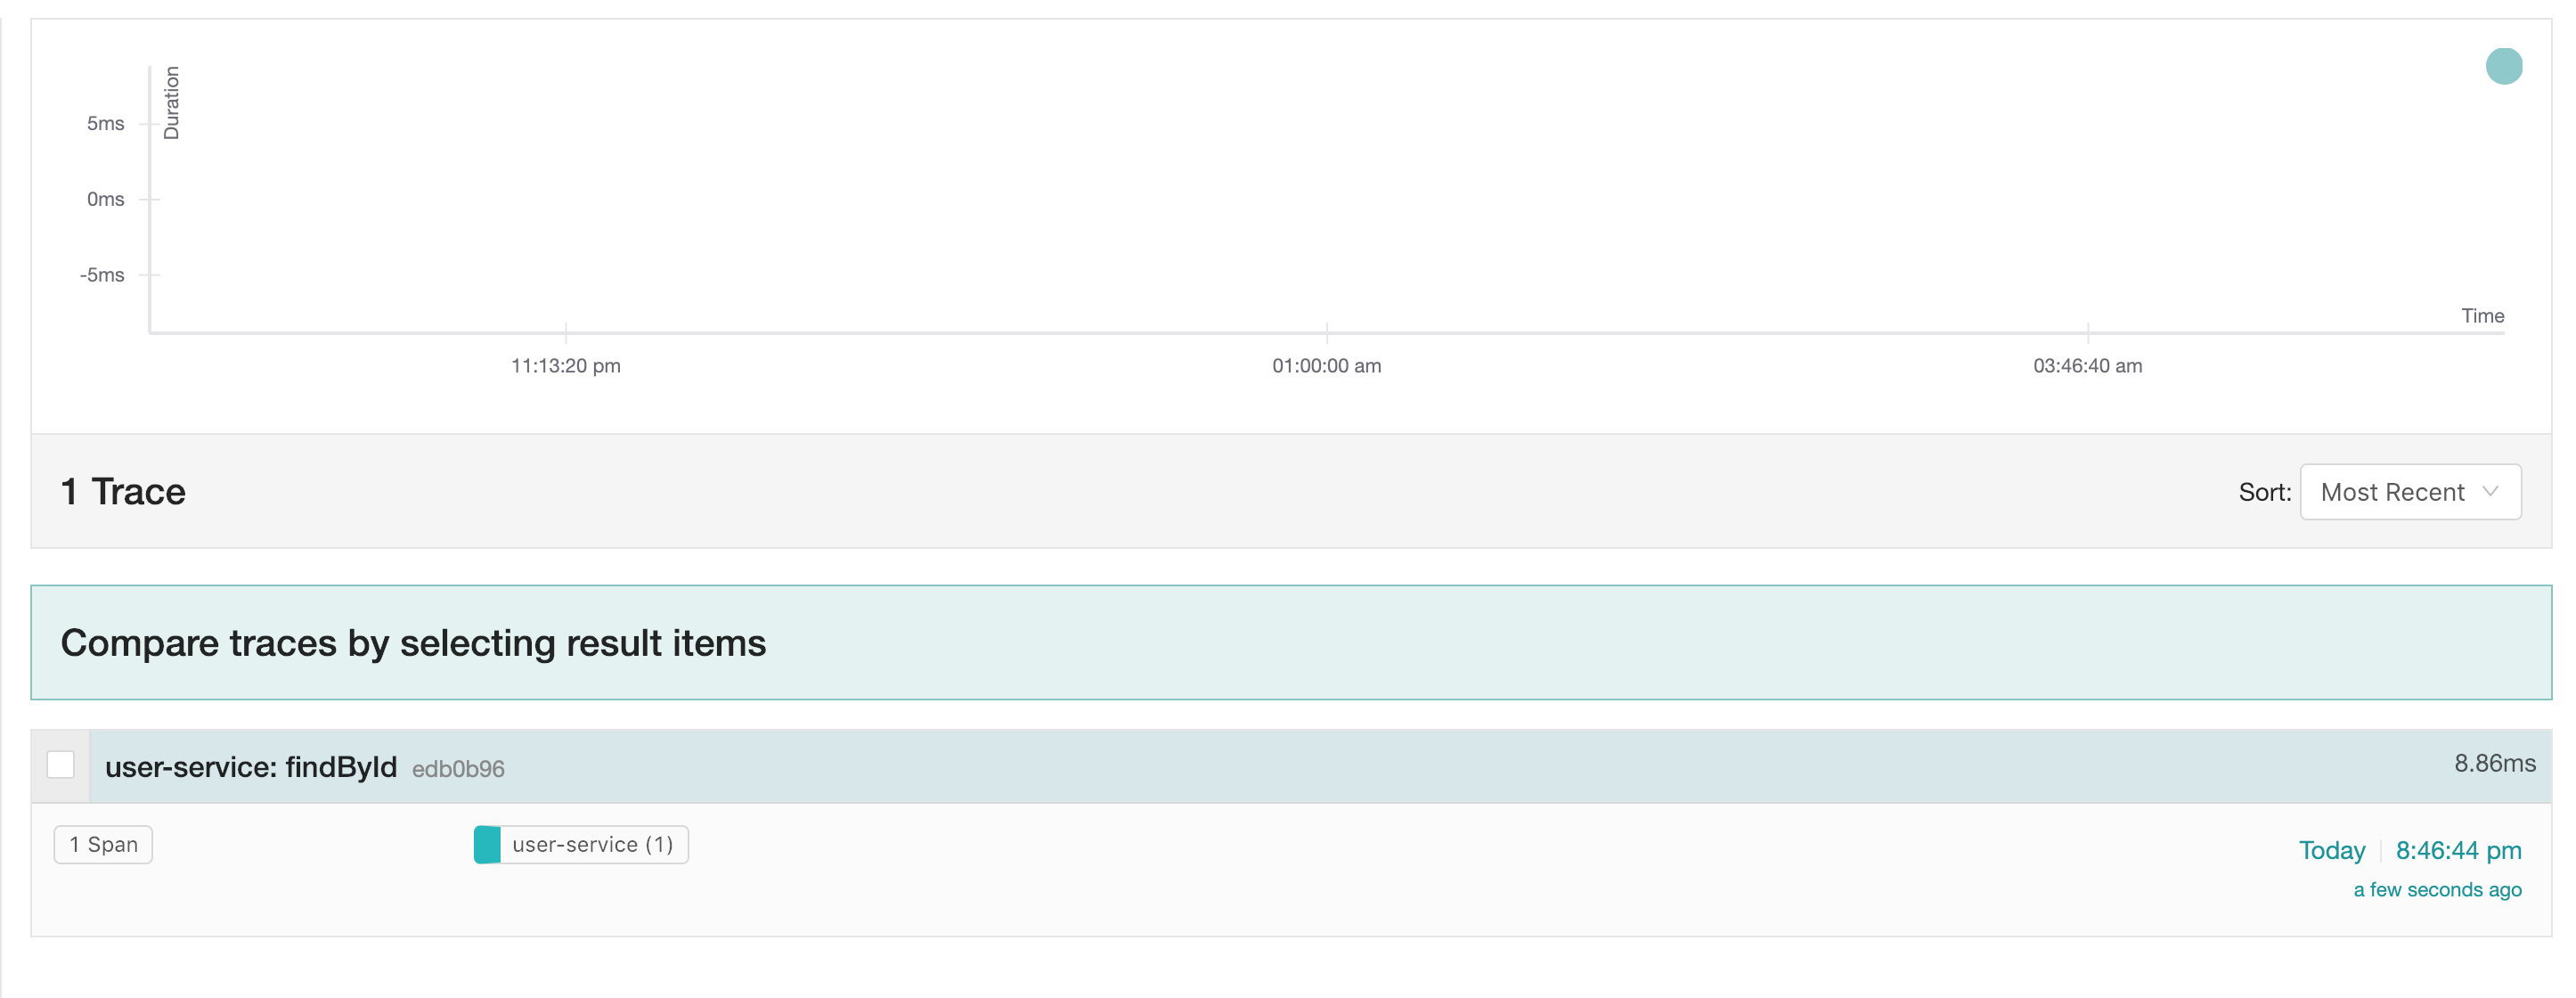
\includegraphics[width=\linewidth]{img/user-service-trace.png}
	\caption{De user-service trace werd gegenereerd en is zichtbaar in Jaeger.}
	\label{fig:user-service-trace}
\end{figure}

\subsection{OpenCensus}
We gaan nu kijken hoe we dezelfde functionaliteit kunnen verkrijgen met gebruik van OpenCensus. Om dit te bereiken dienen we enkele aanpassingen door te voeren aan ons project. We vertrekken echter van een kopie van het OpenTracing project, zo kunnen we later nog aanpassingen maken aan beide projecten indien gewenst.

We navigeren in een terminal naar de directory die 1 niveau hoger ligt van waar onze root pom van OpenTracing zich bevindt en voeren volgend commando uit:
\begin{list}{}{}
	\item \code{cp opentracingparent opencensusparent}
\end{list}
\subsubsection{Root project aanpassen}
We gaan eerst onze dependencies aanpassen in onze root pom. We vervangen alle dependencies die betrekking hebben tot OpenTracing door de OpenCensus dependencies, \code{opencensus-api} en \code{opencensus-impl}. De community heeft een library geschreven om op een eenvoudige manier spring frameworks te instrumenteren met spans. We voegen dus ook de \code{opencensus-contrib-spring} dependency toe. Ook hier gaan we weer met Jaeger werken, we moeten dus de \code{opencensus-exporter-trace-jaeger} dependency toevoegen. Verder passen we onze eigen dependency aan voor de tracing configuratie. We geven in dit geval gewoon een zinnigere naam aan de configuratie module.
\codefragment{xml}{../opencensusparent/pom.xml}{De root pom voor OpenCensus project}{lst:opencensuspom}

\subsubsection{Tracing configuratie module aanpassen}
We voorzien de pom van de juiste dependencies en we passen de naam van onze module aan analoog met de root pom.
\codefragment{xml}{../opencensusparent/opencensus-configuration/pom.xml}{De juiste dependencies werden toegevoegd en de naam van de module werd gewijzigd}{lst:opencensusconfigpom}

Het bestand \code{JaegerTracer.java} mag verwijderd worden, we hebben dit bij OpenCensus niet nodig. We maken een nieuwe klasse aan. Deze klasse bevat de configuratie voor OpenCensus. 

We zorgen ervoor dat, bij het aanmaken van de klasse door spring, de exporter wordt ge\"{i}nstanti\"{e}erd. Hiervoor hebben we enkele variabelen nodig zodat we via omgevingsvariabelen de configuratie desgewenst kunnen aanpassen. We geven volgende variabelen mee, \code{serviceName} \code{jaegerAgentHost} en \code{jaegerAgentPort} en voorzien een zinnige default waarde voor het geval er geen waarde voor de variabele werd gevonden\footnote{Aangezien de application name voor spring boot altijd moet voorzien zijn geven we hier geen default waarde mee}.

Daarnaast gaan we ook bepalen wat de sampling strategie is. Ook hier hebben we een omgevingsvariabele toegevoegd, namelijk \code{jaegerSamplerParam}. Aan de hand van deze waarde gaan we de sampling strategie bepalen en de correcte sampler instanti\"{e}ren.

Als laatste stap voorzien we een bean van de \code{CensusSpringAspect} klasse. Dit is de klasse die ervoor zal zorgen dat we onze code kunnen annoteren met de \code{@Traced} annotatie. Om ervoor te zorgen dat de bean word opgepikt door spring voorzien we de klasse van de \code{@Configuration} annotatie en de \code{@EnableAspectJAutoProxy} annotatie.
\codefragment{java}{../opencensusparent/opencensus-configuration/src/main/java/be/hogent/distributedtracing/OpenCensusConfiguration.java}{De configuratie klasse voor OpenCensus}{lst:opencensusconfig}

\subsubsection{User service aanpassen}
Het enige wat we in de pom van deze module moeten aanpassen is de verwijzing naar onze eigen dependency van de opencensusconfiguration module.
\codefragment{xml}{../opencensusparent/user-service/pom.xml}{De pom voor de user service. Enkel de dependency werd veranderd.}{lst:userserviceopencensuspom}

In de \code{UserService} klasse dienen we enkel de klasse te veranderen in de \code{@Import} annotatie. We veranderen dit in \code{@Import(OpenCensusConfiguration.class)}. De rest blijft ongewijzigd.
\codefragment{java}{../opencensusparent/user-service/src/main/java/be/hogent/distributedtracing/UserService.java}{De aangepaste UserService klasse}{lst:userserviceopencensus}

Door gebruik te maken van de \code{opencensus-contrib-spring} library, zijn de wijzigingen in de \code{UserController} klasse nu ook triviaal. We dienen enkel de annotatie \code{@Traced} toe te voegen aan onze endpoint methode.
\codefragment{java}{../opencensusparent/user-service/src/main/java/be/hogent/distributedtracing/controllers/UserController.java}{In de UserController klasse werd enkel een annotatie toegevoegd.}{lst:usercontrolleropencensus}

\subsubsection{Omgeving opstarten en verifi"eren}
Voor het opstarten van de omgeving kunnen we analoog te werk gaan zoals beschreven bij de OpenTracing implementatie. Doordat we dezelfde variabelen gebruiken voor de Jaeger configuratie volstaat het zelfs om in de directory waar de docker compose file staat het commando \code{docker-compose up} uit te voeren.

Ook voor de verificatie gaan we analoog te werk. Eens we de stappen uitgevoerd hebben zien we inderdaad dat ook hier de traces correct worden gepropageerd naar Jaeger.